\documentclass[11pt, a4paper]{article} 

% Packages
\usepackage[fleqn]{amsmath} % fleqn: flush left equations <-- Left-flush equations
\usepackage{graphicx}

% Format
\usepackage[margin=2cm, top=2cm]{geometry}

% Heading
\title{\bf Design 4-5\\[1ex]
\rm\normalsize CS202 Programming Systems, Summer 2020 }
\date{\normalsize Due: July, 13, 2020}
\author{\normalsize Armant Touche}

\begin{document}

\vspace{0cm}\maketitle 

\section*{UML \#4-5 Diagram:}

            \begin{center}
            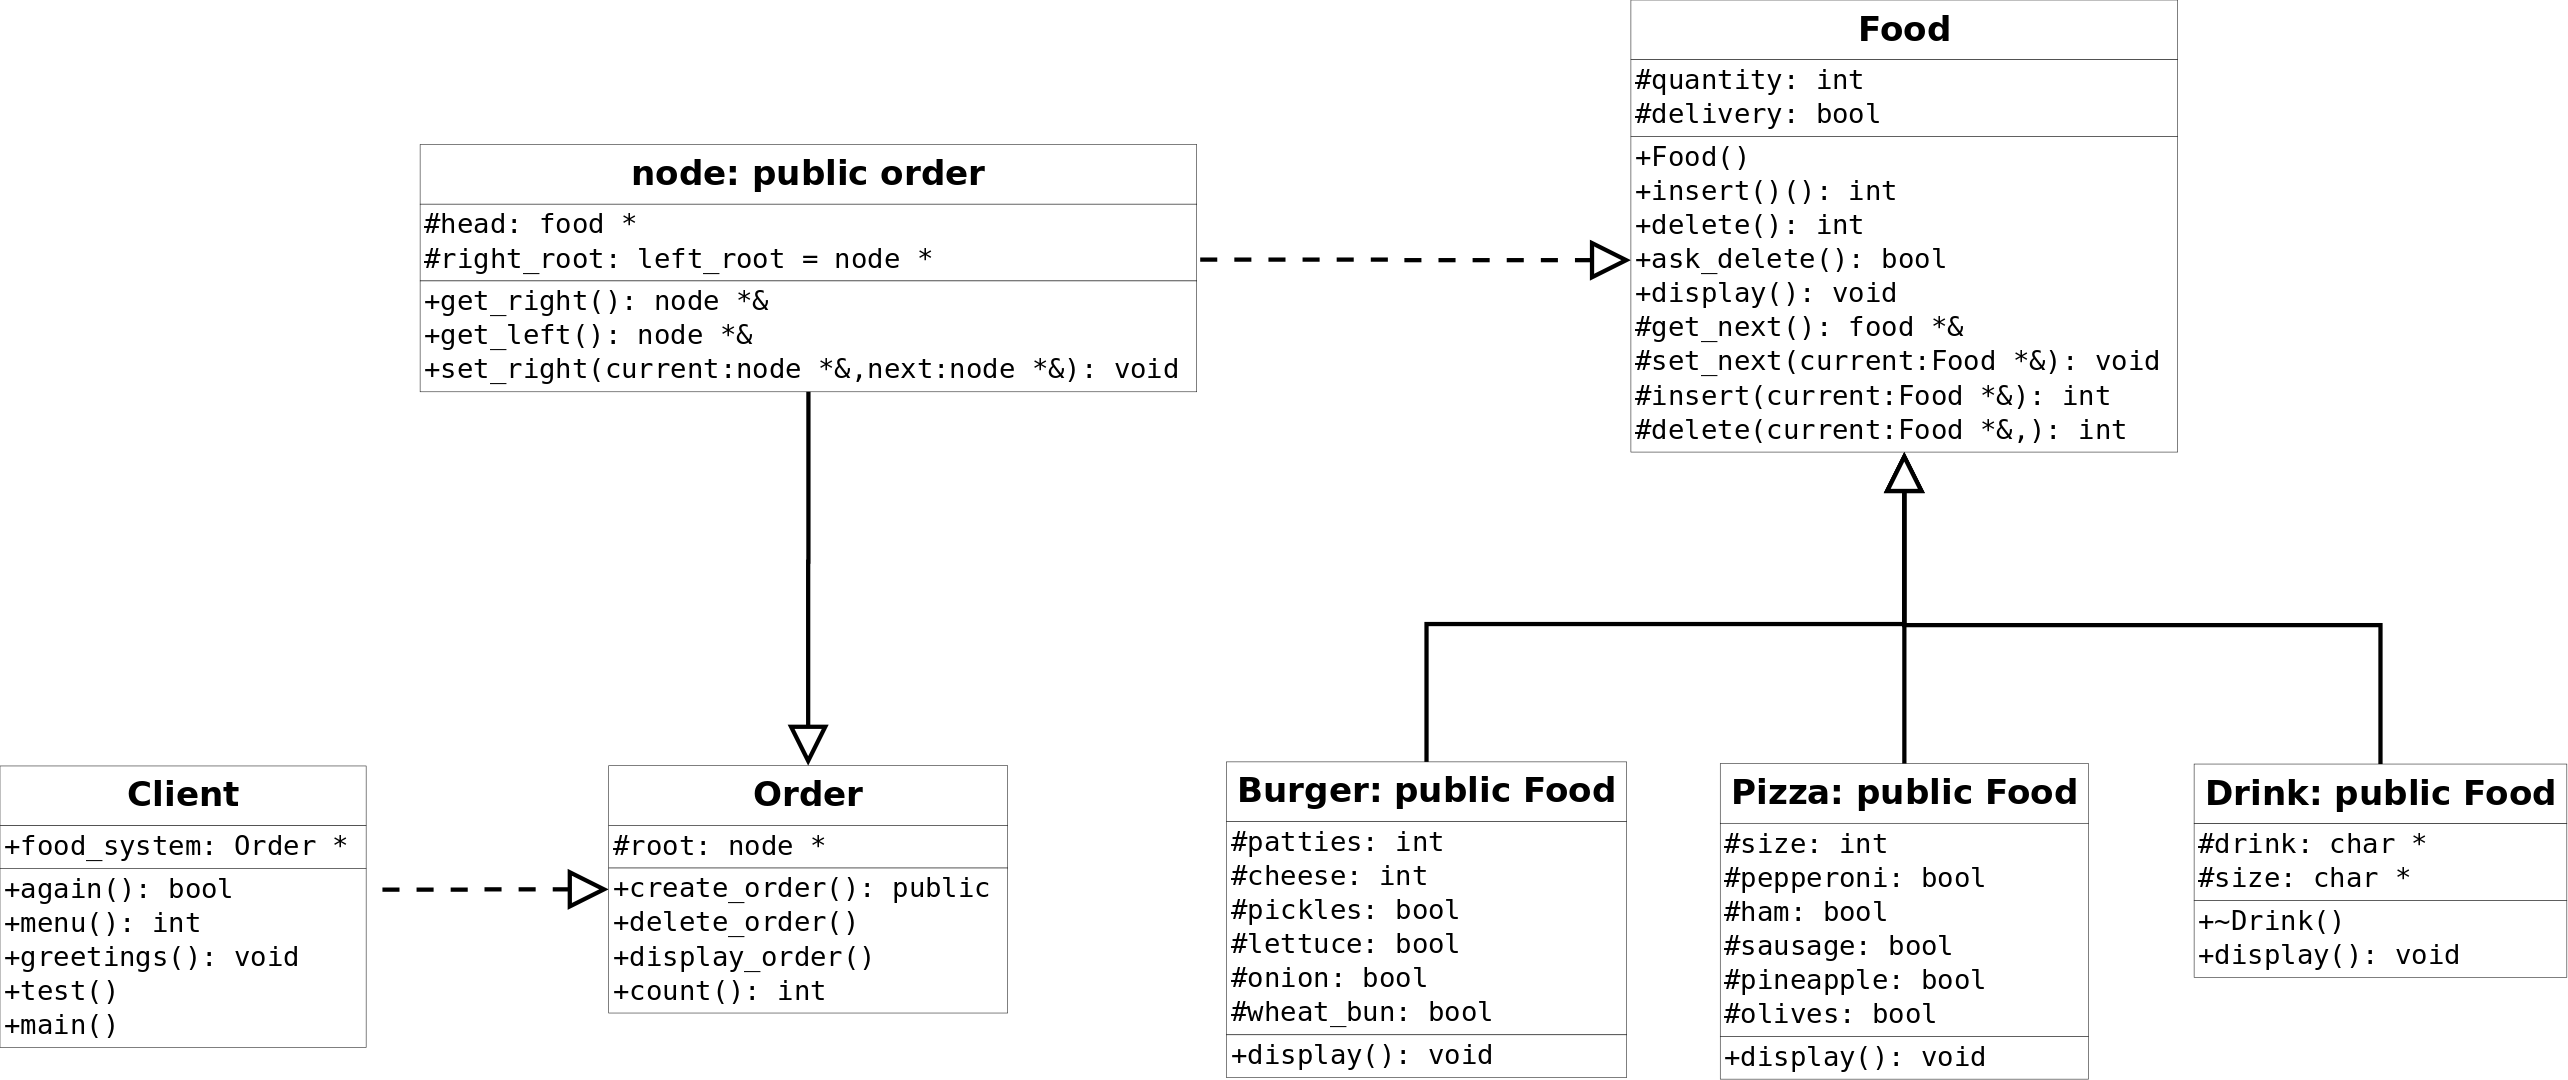
\includegraphics[width=.8\textwidth]{uml4}
            \end{center}

\section*{Write-up:}
For this assignment, we are design and implement a food ordering system where the choices range from three items of our choice. The three items I choose for the food-ordering system was burgers, pizza, and a drink which will be the derived classes. Their parent will be the food class which constitutes a single-inheritance hierarchy. I will first set out implement this hierarchy in Java because I feel I will be spending most of my time implementing the corresponding data structures. To more easily implement the data structure, I will encapsulate a food pointer in a node class which will manage the binary search tree. Also, the food class itself will manage the linear linked list of similar food orders. For sorted purposes, I will sort the linear linked list by most recently added. The binary search tree will be sorted by class type but I do not know if that is sufficient because there would be only three nodes in the binary search tree. For the fifth program, I also do not know how sorting would take place since I have to implement balancing 2-3 tree. I will be putting a lot of hours into these last two programs but with the integrated development environment, there will be a lot of warnings to be had. Coding in an IDE will probably make the implementation much easier but after going through the hard concepts, I feel Karla has set us up for success. The node class for program four and five will be the class managing the trees so my object oriented design will be very similar in each program. My UML didn't reflect what will be done with program five but I feel the hierarchy won't change and the "has a" relationship will not change either. For program five, I will probably have more fields for the added customisation required for program five and will also need to add more methods to account for more functionality. The client class will be the main driver for testing and using the Food order system. The client will have a instance of the Food order system in it's data field section. I will be implementing and testing each of the classes' method along the way. In each class there will exist a test method that be used to test small implementations here and there. For program five, I will have to write data to an external file which should be interesting. Probably in my order class, the method for handling the external data file will be placed there since that will be the hub of all the activity taking place in the programs. The external data file method isn't reflected in the UML but that is because I never dealt w/ I/O in Java. I am not even sure what the library that require to file I/O is. I also wouldn't know how it works but I suspect I will be Googling a lot and visiting Stack Overflow a lot for these two programs. I will have to implement dynamic binding within the single-inheritance hierarchy but that shouldn't be hard since polymorphism in Java isn't restricted to a single class scope like C++. Some function to overload would be display, ask to delete, and insert. The Food class will act as the "glue" and the function being overloaded will be pure virtual function in the base class. In my case, the Food class will be the Abstract Base Class containing pure virtual methods. For program five, I do not know what will need to be changed to accommodate the requirements but I sure homework recitation will be useful in pointing me in the right direction for program number five.

\end{document}
